\documentclass{resume} % Use the custom resume.cls style

\usepackage[left=0.75in,top=0.6in,right=0.75in,bottom=0.6in]{geometry} % Document margins
\usepackage{xcolor}
\usepackage{hyperref}
\hypersetup{
    colorlinks=true,
    linkcolor=blue,
    filecolor=magenta,      
    urlcolor=teal,
}
\usepackage{graphicx}
\newcommand{\tab}[1]{\hspace{.2667\textwidth}\rlap{#1}}
\newcommand{\itab}[1]{\hspace{0em}\rlap{#1}}
\name{Emilio Berti} % Your name
\address{
    \centering
    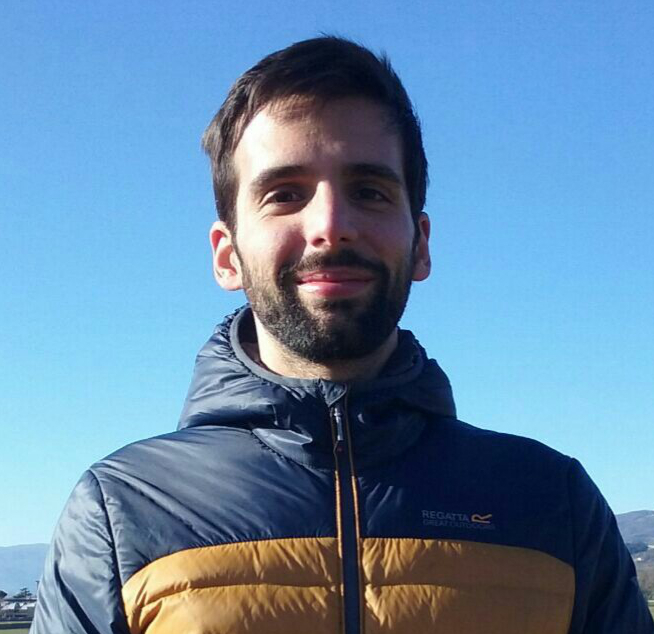
\includegraphics[width=0.25\textwidth]{Emilio.jpg}
} % Your address
%\address{123 Pleasant Lane \\ City, State 12345} % Your secondary addess (optional)
\address{(+45) 266 54 662 \\ emilio.berti.academia@gmail.com} % Your phone number and email

\begin{document}

\begin{rSection}{Sommario}
Nato a Prato nel 1990, sono un ecologo teorico con forte abilit\`{a} matematiche e computazionali.
Dopo aver ottenuto Laurea Triennale e Magistrale dall'Unviersit\`{a} di Firenze, mi sono spostato in Danimarca, dove ho conseguito un PhD dall'Univerit\`{a} di Aarhus nel 2020.
Lo stesso anno, mi sono trasverito a Lipsia, in Germania, per un ruolo di PostDoc al Centro Tedesco per la Ricerca Integrativa sulla Biodiversit\`{a} (iDiv).
La mia ricerca si focalizza su questioni theoriche nel campo della macroecologia e biogeografia ed \`{e} finalizzata a comprendere fenomeni ecologici complessi e promuovere il ripristino della biodiversit\`{a}.
\end{rSection}

\begin{rSection}{Storia lavorativa}

{\bf Ricercatore PostDoc} \hfill {\em Ottobre 2020 -- Presente}\\
Theory in Biodiversity Science\\
German Centre for Integrative Biodiversity Research (\textsc{iDiv})\\
Leipzig, Germania

{\bf Consulente scientifico} \hfill {\em Maggio 2020 -- Luglio 2020}\\
Department of Bioscience\\
Aarhus University\\
Aarhus, Danimarca

{\bf Insegnante assistente} \hfill {\em Febbraio 2017 -- Aprile 2020}\\
Department of Biology\\
Aarhus University\\
Aarhus, Danimarca

\end{rSection}

\begin{rSection}{Educazione}
{\bf PhD} \hfill {\em Febbraio 2017 -- Giugno 2020} 
\\ Section of Ecoinformatics and Biodiversity
\\ Department of Biology
\\ Aarhus University
\\ Aarhus, Danimarca\\
\\ {\bf Studente PhD in visita} \hfill {\em Autunno 2018}
\\ Department of Ecology and Evolution
\\ University of Chicago
\\ Chicago, IL\\
\\ {\bf MSc cum laude in Biologia} \hfill {\em 2013 -- 2016}
\\ Dipartimento di Biologia
\\ Universit\`{a} di Firenze
\\ Firenze, Italia\\
\\{\bf BSc in Biologia} \hfill {\em 2009 -- 2012}
\\ Dipartimento di Biologia
\\ Universit\`{a} di Firenze
\\ Firenze, Italia\\
\vskip3ex
\end{rSection}

\begin{rSection}{Corsi post-laurea}
{\bf ``Collaboration and Competition in Science''} \hfill {\em 2021}\\
Jena, Germania -- Insegnante: Nina Bessing\\
{\bf ``Species Distributions Modelling''} \hfill {\em 2019}\\
Evora, Portogallo -- Insegnante: Prof. Miguel Ara\'{u}jo \& Dr. Babak Naimi\\
{\bf ``Megafauna ecology -- shaping past, present and future ecosystems.''} \hfill {\em 2019}\\
Aarhus, Danimarca\\
{\bf ``Mixed models''} \hfill {\em 2019}\\
Aarhus, Danimarca -- Insegnante: Prof. Rodrigo Labouriau\\
{\bf ``Writing and Speaking Science in English for Biology Students''} \hfill {\em 2019} \\
Aarhus, Danimarca -- Insegnante: Prof. Brian Sorrell \\
{\bf ``Ecosystem roles of megafauna in the past, present, and future''} \hfill {\em 2017}\\
Aarhus, Danimarca\\
{\bf ``Mediterranean School of Complex Networks (MSCx)''} \hfill {\em 2017} \\
Salina, Italia
\end{rSection}

\begin{rSection}{Insegnamenti \& organizzazione workshops}
{\bf Insegnante assistente} \\
Meta-analisi per studi sulla Biodversit\`{a} (2021)\\
Statistica e modelli geospaziali (2019)\\
Ecologia comportamentale (2018, 2019)\\
Geographic Information System (2017)\\
{\bf Organizzazione workshops}\\
``Cleaning online repository data for use in biogeography and macroecology'' (2019)\\
``Running a species distribution model in R.'' (2019)\\
``A (very) gentle introduction to Linux.'' (2019)
\end{rSection}

% \begin{rSection}{References}
% \textbf{Jens-Christian Svenning} (Professor)\\
% Aarhus University, Department of Biology, Ecoinformatics and Biodiversity\\
% E-mail: svenning@bios.au.dk
% Phone: +45 289 92 304

% \textbf{Robert Buitenwerf} (Assistant Professor)\\
% Aarhus University, Department of Biology, Ecoinformatics and Biodiversity\\
% E-mail: buitenwerf@bios.au.dk\\
% Phone: +45 871 54 346

% \textbf{Giacomo Santini} (Assistant Professor)\\
% Florence University, Department of Biology\\
% E-mail: giacomo.santini@unifi.it\\
% Phone: +39 055 45 74 721
% \end{rSection}

\begin{rSection}{Pubblicazioni}
% \vspace{4ex}\hfill{\em 2020}\\
\textbf{Berti, E.} \& Svenning, J.C. (2020). Megafauna extinctions have reduced biotic connectivity worldwide. \textit{Global Ecology and Biogeography}. DOI: \href{https://doi.org/10.1111/geb.13182}{10.1111/geb.13182}.

\textbf{Berti, E.}, Monsarrat, S., Munk, M., Jarvie, S., \& Svenning, J.C. (2020). Body size is a good proxy for vertebrate charisma. \textit{Biological Conservation}. DOI: \href{https://doi.org/10.1016/j.biocon.2020.108790}{10.1016/j.biocon.2020.108790}.

\textbf{Berti, E.}, Davoli, M., \dots \&Vollrath, F. (2021). Enerscape. \textit{Methods in Ecology and Evolution}. DOI: \href{}{}.
\end{rSection}

\begin{rSection}{Links}
\begin{minipage}{0.5\textwidth}
\begin{itemize}
    \item \href{https://scholar.google.com/citations?user=5KPh-oUAAAAJ&hl=en}{Google Scholar}
    \item \href{https://emilio-berti.github.io/}{Webpage personale}
    \item \href{https://orcid.org/0000-0001-9286-011X}{ORCiD}
\end{itemize}
\end{minipage}
\begin{minipage}{0.5\textwidth}
\begin{itemize}
    \item \href{https://www.linkedin.com/in/emilio-berti-55a348146}{LinkedIn}
    \item \href{https://github.com/emilio-berti}{GitHub}
\end{itemize}
\end{minipage}
\end{rSection}

\end{document}
